\chapter{Topology in non-Hermitian systems}
\label{ch:nh}
Almost all axioms of quantum mechanics are rooted in fundamental physical requirements. For instance, the time evolution of a quantum system has to be governed by a unitary operator $e^{-\mathrm{i}Ht}$, because it conserves probability. Conjointly, the energy spectra have to be bounded from below, which means that a stable lowest-energy state exists, and has to be real-valued as they correspond to the possible outcomes of a measurement. These prerequisites are instantaneously fulfilled by assuming that the Hamiltonian $H$ describing the dynamics of a system is Hermitian, \ie equal to its adjoint, $H =  H^{\dagger}$. However, Bender and Boettcher~\cite{BenderPT1998} pointed out that Hermiticity is a sufficient, but not a \emph{necessary} condition that guarantees the eigenvalues to be real. It can actually be relaxed to a weaker condition, where the combined action of the parity $\mathcal{P}$ and the time-reversal $\mathcal{T}$ operators, $[H, \mathcal{PT}] = 0$\footnote{Suppose the Hamiltonian $H$ is expressed in terms of the position $\mathbf{x}$ and momentum $\mathbf{p} = - \mathrm{i} \nabla$ operators, $H = \mathbf{p}^2 + V(\mathbf{x})$, where $V(\mathbf{x})$ is a potential energy. The space reflection operator $\mathcal{P}$ flips the sign of the $\mathbf{x}$ and $\mathbf{p}$ operators, $\mathcal{P}: \mathbf{x} \rightarrow - \mathbf{x}, \, \mathbf{p} \rightarrow - \mathbf{p}$, while the time-reversal operator $\mathcal{T}: \mathbf{x} \rightarrow \mathbf{x}, \, \mathbf{p} \rightarrow - \mathbf{p}, \, \mathrm{i} \rightarrow - \mathrm{i}$. If the Hamiltonian has to be $\mathcal{PT}$-symmetric, then the potential $V(\mathbf{x})$ satisfies $ \mathcal{PT} V( \mathbf{x} )\mathcal{TP} = V^* (- \mathbf{x} ) = V (\mathbf{x} )$. This condition implies that $V(\mathbf{x})$ is in general a complex function where the real part is an even function and the imaginary is an odd function of $ \mathbf{x}$.}, constrains the realness of the energies. 

$\mathcal{PT}$-symmetric systems can be regarded as systems that interact diffusively with the environment as their potential energy is often complex. A potential with a positive imaginary part characterizes a system which gains energy from its environment. Conversely, a potential with a negative imaginary part corresponds to a system losing energy. In the presence of the $\mathcal{PT}$-symmetry, gain and loss are balanced and the system can reach an equilibrium state~\cite{Bender_2015}. This initial proposal of $\mathcal{PT}$-symmetric systems was firstly extended to the field of optics~\cite{Zyablovsky_2014, El-Ganainy2018, ozdemir2019}, where one can straightforwardly realize the $\mathcal{PT}$-symmetry condition by coupling two identical waveguides, one with gain and the other with the equal amount of loss. Then, the $\mathcal{P}$-symmetry interchanges the subsystems, while the $\mathcal{T}$-symmetry swaps between gain and loss. In parallel, $\mathcal{PT}$-symmetry has been exploited in other experimental setups, including electronics~\cite{PhysRevA.84.040101} or metamaterials~\cite{PhysRevA.87.053824,PhysRevLett.113.023903}. 

$\mathcal{PT}$-symmetric Hamiltonians can be thought as a special class of the general non-Hermitian (nH) formalism in which the physics of open systems, \ie systems that do not conserve energy or particle number, is captured at an \emph{effective} level. The concept of non-Hermitian effective Hamiltonians dates back to the studies on alpha decay~\cite{Gamow1928}. It was shown that a particle may escape the nucleus at a tunnelling rate given by its complex-valued eigenenergies with the real (imaginary) part of these energies being associated with the levels (widths) of the nuclear resonances. Later on, complex, non-Hermitian potentials were introduced to describe the scattering between nuclei and neutrons~\cite{PhysRev.96.448}. These approaches, though, are rather phenomenological than fully mathematically justified. A more careful treatment of dissipative systems coupled to the environment can be for instance based on Lindblad master equations~\cite{Lindblad1976}, originally introduced in the context of quantum optics and spin systems. Assuming an open system to be described by a density matrix $\rho$, the non-unitary (but Markovian) time evolution of $\rho$ is then given by the equation $\dot{\rho} = - \mathrm{i} [H, \rho] + \sum_{\mu} (2 L_{\mu} \rho L_{\mu}^{\dagger} - \lbrace L_{\mu}^{\dagger} L_{\mu}, \rho \rbrace  ) = \mathcal{L} [\rho]$ with $ \mathcal{L} [\rho]$ as a superoperator called Lindbladian\footnote{A superoperator is a map acting on operators. Here, the superoperator $\mathcal{L}$ connects the initial density matrix to the time-evolved one, $\rho(t) = \rho (0) +  \int_0^t \mathcal{L} (\rho(t')) dt'$. $\mathcal{L}$ has to be positive, linear, and preserve trace and Hermiticity.}~\cite{breuer2002theory}. $H$ is a Hermitian Hamiltonian generating unitary dynamics, $L_{\mu}$ denotes the Lindblad operators (loss channels such as spin flips due to the coupling to the environment) and each $ L_{\mu} \rho L_{\mu}^{\dagger}$ term induces a quantum jump. The short-time evolution (before the occurrence of a quantum jump) can be then written as $\dot{\rho} = - \mathrm{i} \, (H_{\mathrm{eff}} \rho - \rho H_{\mathrm{eff}}^{\dagger})$ with the effective non-Hermitian Hamiltonian $H_{\mathrm{eff}} = H - \mathrm{i} \sum_{\mu} L_{\mu}^{\dagger}   L_{\mu}$. Other powerful methods, such as the idea of Feynman and Vernon~\cite{FEYNMAN2000547} explaining the effects of an environment on the system in terms of an influence functional or with Keldysh diagrammatic technique~\cite{keldysh1965diagram}, are also widely employed. However, the high complexity of aforementioned tools usually reduces their applicability and non-Hermitian effective Hamiltonians can then serve as a simple, macroscopic description.

It is only recently that the interplay between non-Hermiticity and topology has received immense interest. Topological phases supported by non-Hermitian Hamiltonians yields qualitatively novel phenomena~\cite{PhysRevX.8.031079,foatorres19jpm}, such as the occurrence of stable defective degeneracy points called exceptional points~\cite{lee19prl133903,alvarez18prb121401}. In two-dimensional systems~\cite{PhysRevLett.120.146402}, these exceptional points can be connected by bulk Fermi arcs~\cite{Zhou1009}, which are usually only observed in 3D Weyl semimetals. Another exotic feature resolved through the band theory description of open systems is the non-Hermitian skin effect~\cite{Shunyu2018prl}, where \emph{all} of the eigenstates of a one-dimensional system can localize at one of its boundaries. The skin effect is a manifestation of the breakdown of bulk-boundary correspondence, a core principle of topological band theory in closed systems~\cite{XiongBBCbreakdown2018,bbbc,PhysRevB.99.201103,BorgniaCitationRequest}. The non-Hermitian skin effect has been discussed in one-dimensional systems, and was initially assumed to require a non-reciprocal Bloch Hamiltonian usually realized through asymmetric, direction-dependent hoppings. Reciprocal versions of the one-dimensional skin effect can be constructed by introducing additional degrees of freedom. Their protection against hybridization is realized by demanding additional symmetries such as mirror symmetry~\cite{SchnyderPRB2019,okuma2019topological}. In this work, we present a generalized skin effect in reciprocal systems, that is enabled by non-Hermiticity in dimensions higher than one. For simplicity, we constrain ourselves to two spatial dimensions. The basic idea is that, while a reciprocal model cannot localize all of its OBC eigenstates at just one boundary, it may still do so for states of a particular boundary momentum. Reciprocity then implies that eigenstates at opposite momenta are localized at opposite boundaries. 

The reciprocal skin effect dramatically expands the scenarios in which anomalous extensive skin mode localization~\cite{PhysRevB.99.201103} can be found in nature. As a paradigmatic experimental realization within a framework of high accessibility and tunability, we implement the reciprocal skin effect within a topolectrical circuit setup. Similar to many other classical platforms of synthetic topological matter, this roots in the insight that phenomena related to the Berry phase~\cite{berry84,ZakPhase2} can be also observed in classical physics~\cite{Haldane:86}, since they do not concern phase space, but parameter space. The realization of topological phases in photonic~\cite{PhysRevLett.100.013904}, mechanical~\cite{lubensky,PhysRevLett.114.114301} and electrical systems~\cite{ningyuan2015time,PhysRevLett.114.173902,hu2015measurement,LeeTopolectrical18,imhof,PhysRevLett.122.247702,knots,LeeTopolectrical18,interf-nh-ezawa,nh-haldane-ezawa,wang2019topologically} demonstrates this connection between topological aspects of quantum and classical systems. The non-Hermitian band theory of open quantum systems can similarly be mirrored by classical systems that involve gain and loss. Electric circuits whose circuit Laplacian~\cite{LeeTopolectrical18} is modeled in analogy to a quantum Bloch Hamiltonian are particularly suited for this: loss and gain can be directly implemented by resistors and active circuit elements~\cite{PhysRevLett.122.247702}, respectively, while Hermitian hybridization elements are realized by inductive and capacitive links between circuit nodes.  We design, describe, and measure~\cite{PhysRevB.99.161114} a non-Hermitian topolectrical circuit that displays, among exceptional points, the reciprocal skin effect, and is built entirely from capacitors, inductors, and resistors, \emph{without} the need for non-reciprocal active elements such as operational amplifiers. Being a passive circuit network, its convenient translation into alternative platforms of synthetic topological matter promises ubiquitous realizations and applications in optics, mechanics, and acoustics. The structure of this Chapter is following: in Section~\ref{sec:nh-bands}, we introduce the basic notions underlying the non-Hermitian band theory and present in more detail the unique non-Hermitian phenomena, without any Hermitian counterparts. We then move to discussing the quantum lattice $\pi$-flux model in Section~\ref{sec:nh-piflux} and show how the novel features arise due to the additional non-Hermitian terms. Finally, Section~\ref{sec:topocircuit} presents a connection between the model within tight-binding approximation and a circuit Laplacian used for designing the topolectical circuit, together with the experimental results.

\section{Non-Hermitian topological band theory}
\label{sec:nh-bands}
Non-Hermiticity has a profound effect on topological band theory. Some nH topological systems can be regarded as generalizations of well-studied topological phases, both gapped and gapless, described by Hermitian Hamiltonians. Examples include nH extensions of Chern insulators~\cite{PhysRevLett.120.146402,PhysRevLett.121.136802}, Weyl semimetals~\cite{PhysRevResearch.1.012003}, Floquet systems~\cite{PhysRevB.101.045415, PhysRevResearch.2.023235} or higher-order TIs~\cite{PhysRevLett.122.076801, PhysRevB.99.201411, PhysRevB.99.081302}. But more importantly, nH topological systems exhibit novel phenomena which are not observed in the Hermitian limit. The goal of this Section is to bring up the essential notions required to define band topology in nH Hamiltonians, which are often differently formulated than in Hermitian systems. In particular, non-Hermiticity enriches the standard ten-fold classification as new types of symmetries arise. On that line, we continue with discussing the exceptional structures - spectral degeneracies associated with a Hamiltonian defectiveness that solely origin from the non-Hermiticity. The lack of a complete basis set affects the eigenstate localization properties and, in general, allows to pile up all states at the same edge of a system. Finally, the sensitivity of the eigenstates of nH Hamiltonians to the boundary conditions leads to the revision of the bulk-boundary correspondence principle. For more information, we refer the reader to the excellent Refs.~\cite{bergholtz2019exceptional, ashida2020nonhermitian}.

\subsection{Complex energy gap and winding number}
As the eigenvalues of nH Hamiltonians are in general complex, the definition of the energy gap is no longer unique. Various extensions of this concept are possible, such as identifying the bands to be separable or inseparable~\cite{PhysRevLett.120.146402}\footnote{Consider a nH Hamiltonian with PBC, whose eigenstates are Bloch states with energies $E_n( \mathbf{k} )$ depending on the crystal momentum $\mathbf{k}$ in the BZ. The $n$-th band is said to be \emph{separable} if its energy $E_n (\mathbf{k}) \neq E_m (\mathbf{k})$ for all $m \neq n$ and $\mathbf{k}$. Then, the $n$-th band is \emph{isolated} if $E_n (\mathbf{k}) \neq E_m (\mathbf{k'})$ for all $m \neq n$ and $\mathbf{k}, \, \mathbf{k'}$. If at some momentum $\mathbf{k}$ two or more complex energies are degenerate (so that they have the same real and imaginary parts), then a band is called \emph{inseparable}. Definitions of separable, isolated and inseparable bands are corresponding, respectively, to gapped, fully gapped and gapless bands in Hermitian systems.} and the prohibition of touching a base energy $E_B$, which is typically set to zero~\cite{PhysRevX.8.031079}. The energies can be represented on the complex plane, where the real (imaginary) part of the energy corresponds to the $x$ ($y$) axis (cf. Fig.~\ref{fig:gaps}). In the Hermitian case, the gapped spectrum lies in two segments on the real axis, separated by the imaginary axis and never touching the base energy. Non-Hermitian systems, however, exhibit two type of gaps:

\begin{enumerate}[label=\textbf{\arabic*.}]
\item a \emph{point} gap~\cite{PhysRevX.8.031079}. The eigenvalues may form loops in the complex energy plane and if the base energy $E_B$ lies inside one of the loops, the loop cannot be deformed onto a point without touching the base. This is a genuinely nH case, without any Hermitian equivalent.
\item a \emph{line} gap~\cite{PhysRevX.9.041015, BorgniaCitationRequest} is defined by a line in the complex energy plane, which separates the energy bands. Hermitian systems follow naturally this definition, and nH line-gapped systems share some similarities with Hermitian systems. Models with a line gap always have a point gap.
\end{enumerate}

\begin{figure}[H]
\centering
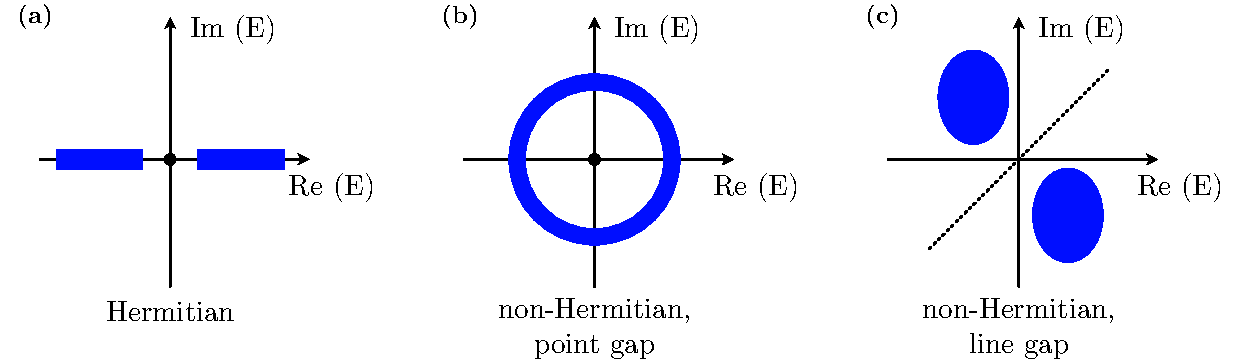
\includegraphics[width=0.95\columnwidth]{nh-gaps.pdf}
\caption[Schematic representation of an energy gap in Hermitian and non-Hermitian Hamiltonians.]{Schematic representation of an energy gap in Hermitian and non-Hermitian Hamiltonians. \textbf{(a)} For Hermitian systems, all energies are represented on the real axis and separated by a gap with the Fermi energy denoted by a black dot. In the non-Hermitian case, the energies can be either separated by \textbf{(b)} a point gap or \textbf{(c)} a line gap.}
\label{fig:gaps}
\end{figure}

In Hermitian systems, a minimal model that can exhibit non-trivial topology has to have at least two bands as the total Berry curvature summed over all bands must be zero. Moreover, topological states are absent in $1D$ systems without enforcing symmetries~\cite{RevModPhys.82.3045, RevModPhys.83.1057}. A hallmark of nH systems is that they can posses some topological features even within a single band. For the one-dimensional nH Bloch Hamiltonian $\mathcal{H} (k)$ with a point gap spectrum, it is possible to define the winding number~\cite{okuma2019topological} (also called vorticity~\cite{PhysRevLett.120.146402})
\begin{equation}
W = \frac{1}{2 \pi \mathrm{i}} \int_{0}^{2 \pi} \, d k \,   \partial_k \log \left[ \det (\mathcal{H}(k) - E_B \, \mathbb{1} ) \right],
\label{eq:nh_winding}
\end{equation}
which measures the number of times the complex eigenenergies encircle $E_B$. Remarkably, this winding number refers only to \emph{eigenvalues}, not eigenvectors, and takes integer values. To illustrate the non-zero winding in a minimal setup, let us consider the Hatano-Nelson model~\cite{hatano-nelson} with asymmetric hoppings $J_R, \, J_L \in \mathbb{R}$
\begin{equation}
H = \sum_i ( J_R \,  c^{\dagger}_{i +1}  c_i + J_L \, c^{\dagger}_i c_{i +1} ), 
\label{eq:hatano-nelson}
\end{equation}
which is non-Hermitian if $J_R \neq J_L^*$. In reciprocal space, the Bloch Hamiltonian has the energy spectrum $E(k) = (J_L + J_R) \cos(k) + \mathrm{i} (J_L - J_R) \sin(k)$. As it is a one-band model, we can replace $\det \mathcal{H} (k)$ term in Eq.~\eqref{eq:nh_winding} by $E(k)$. To compute the winding number $W$, we track how $E(k)$ winds around the base energy $E_B$ (which we take here to be zero) with respect to $k$. When $|J_L| / | J_R | < 1$ ( $>1$), $E(k)$ winds (counter)-clockwise and results in a winding number $-1$ ($+1$). These two phases characterized by $W = \pm 1$ are separated by a topological phase transition at $|J_R| = |J_L|$, where the spectrum touches the base energy.  

\begin{figure}[H]
\centering
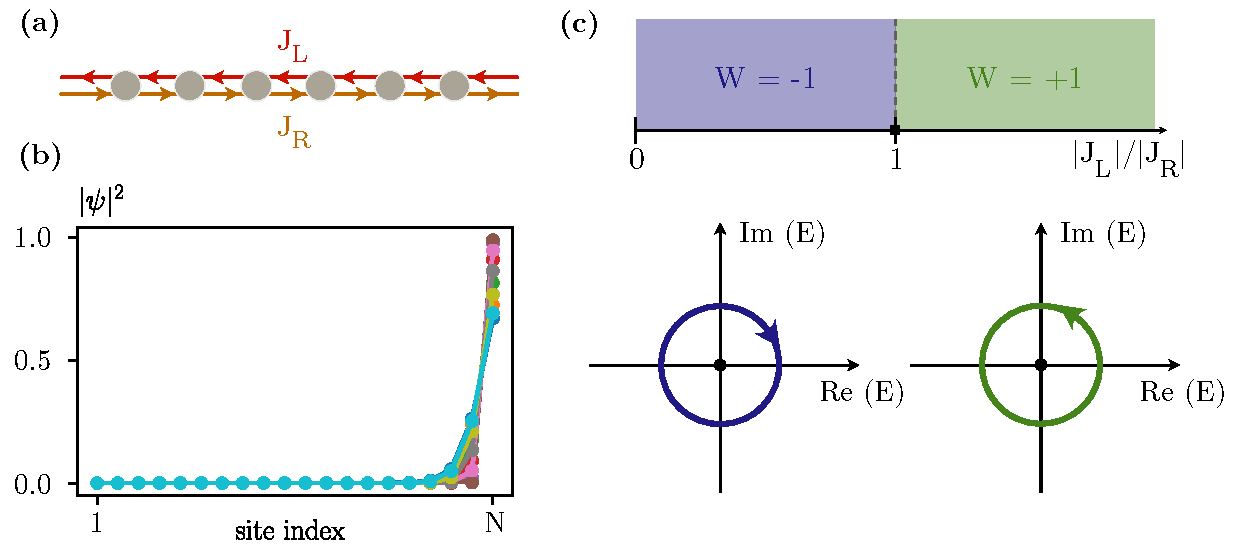
\includegraphics[width=0.95\textwidth]{nh-hatano.pdf}
\caption[The Hatano-Nelson model]{The Hatano-Nelson model. \textbf{(a)} Schematic depiction of a one-dimensional chain with asymmetric hoppings $J_R$ ($J_L$) in the right (left) direction. \textbf{(b)} The Direction-dependent hopping terms induce an anomalous localization of all eigenstates at the edge in a system with open boundary conditions. Here, we set $|J_L| / | J_R | = 0.1$, which leads to the manifestation of the skin effect at the right boundary. \textbf{(c)} The phase diagram as a function of the ratio $|J_L| / | J_R |$. In the range $|J_L| / | J_R | \in [0, 1)$, the winding $W = -1$, while for $|J_L| / | J_R | > 1$, $W = 1$. At $|J_L| / | J_R | =1$, the system undergoes a topological phase transition and all complex energies collapse along a single line crossing the origin. Below, we depict the spectral winding around the base energy. An arrow indicates the direction in which the energies wind as $k$ increases, determining the sign of $W$.}
\label{fig:hatano-nelson}
\end{figure}

In general, the spectral winding number $W$ defined in Eq.~\eqref{eq:nh_winding} allows for a $\mathbb{Z}$ classification and does not require any symmetry. It is in a stark contrast to the winding number in the Hermitian case (discussed in the Chapter~\ref{ch:topo-intro}), which requires chiral symmetry.

\subsection{Biorthogonal quantum mechanics}
Topological invariants such as polarization or Wilson loop can be generalized to the non-Hermitian case by introducing the notion of biorthogonality, which is weaker than the orthogonality observed in the Hermitian limit. Biorthogonality establishes the relationship between the eigenstates of the operator and its self-adjoint. The eigenstates of an operator are not necessarily orthogonal to each other but they are orthogonal to the eigenstates of the self-adjoint of the operator. This is the core of biorthogonal quantum mechanics, which is valid as long as we have no exceptional points and reduces to the standard quantum mechanics in the Hermitian limit. For this part, we closely follow Ref.~\cite{brody2013biorthogonal}. 
A generic nH-Hamiltonian $H$, decomposed into two Hermitian parts $H = H_1  - \mathrm{i} H_2$ with $H_1 = H_1^{\dagger}$ and $H_2= H_2^{\dagger}$, has distinct left $\ket{\psi_L}$ and right $\ket{\psi_R}$ eigenvectors satisfying
\begin{equation}
H  \ket{\psi_{R, i}} = E_i \ket{\psi_{R, i}}, \hspace*{0.5cm} \bra{\psi_{L, i}} H = E_i  \bra{\psi_{L, i}}               \Leftrightarrow H^{\dagger} \ket{\psi_{L, i}} = E_i^*  \ket{\psi_{L, i}}.
\label{eq:schrod-eq}
\end{equation}
In the Hermitian case, the left and right eigenvectors would be equal, $\ket{\psi_{L, i}} = \ket{\psi_{R, i}}$, and a set $\lbrace \ket{\psi_{R, i}} \rbrace$ would form an orthogonal basis. However, if the matrix is nH, the eigenstates are not necessarily orthogonal, \ie the inner product $\braket{ \psi_{R, i} | \psi_{R, j}}$ (and analogously for $\ket{\psi_{L, i}}$) is not zero for all eigenstates
\begin{equation}
\braket{ \psi_{R, i} | \psi_{R, j}} = 2 \,  \frac{ \braket{\psi_{R, i} | H_1 | \psi_{R, j}}} {E^*_i - E_j}  = 2 \,  \mathrm{i} \frac{ \braket{\psi_{R, i} | H_2 | \psi_{R, j}}}{E^*_i - E_j} ,  \hspace*{0.3cm} i \neq j,
\label{eq:biorth_norm}
\end{equation}
where $2 \mathrm{i} H_2 = H^{\dagger} - H$ and $2 H_1 = H^{\dagger} - H$. On the other hand, the basis sets $\lbrace \ket{\psi_L, i} \rbrace$ and $\lbrace \ket{\psi_R, i} \rbrace$ form a biorthogonal basis such that
\begin{equation}
\braket{\psi_{L,i } | \psi_{R,j}} = \delta_{ij}. 
\label{eq:biorth_norm_LR}
\end{equation} 
All the expectation values can be then expressed in terms of a biorthogonal basis, $\braket{\psi_{L, i} | O | \psi_{R,i}}$, for any operator $O$. Conventional Hermitian expressions for topological invariants can then be adapted by replacing the bra states by the left eigenstates and the ket states by the right eigenstates.

\subsection{Symmetry classification}
NH Hamiltonians are not longer equivalent to their self-adjoint representation, which allows for distinct combinations of symmetries generalizing the AZ classification. For instance, the particle-hole symmetry states that $\mathcal{P} H^* \mathcal{P}^{-1} = -H$. In the Hermitian case, complex conjugation coincides with transposition, $H^* = H^{\mathrm{T}}$, and therefore PHS can be also defined as $\mathcal{P} H^{\mathrm{T}} \mathcal{P}^{-1} = -H$. In nH systems, however, these two operations are no longer equivalent and the action of the particle-hole symmetry splits into two different symmetry conditions. A similar situation occurs for the chiral symmetry $\mathcal{C} = \mathcal{PT}$, equivalent to the sublattice symmetry in Hermitian systems. In the absence of Hermiticity, $\mathcal{C}^{-1} H^{\dagger} \mathcal{C} \neq \mathcal{C} H \mathcal{C}^{-1}$. Therefore, non-Hermiticity enables the so-called pseudo-Hermiticity to be a new internal symmetry, defined as $\eta H^{\dagger} \eta^{-1} = H$ with $\eta^2 = 1$. In fact, $\eta$ generalizes the notion of Hermiticity and play a role akin to the parity-time symmetry~\cite{doi:10.1063/1.1418246}. Exhausting all internal symmetries that may appear in nH systems extends the standard 10-fold symmetry classification to 38-fold classification\footnote{A first attempt to classify non-Hermitian random matrices was firstly proposed by Bernard and LeClair~\cite{Bernard_2002}, in which they recognized four fundamental classes of symmetries
\begin{itemize}[noitemsep,topsep=0pt]
\item C symmetry: $c H^{\mathrm{T}} c^{-1} = \varepsilon_c H, \hspace*{0.5cm} c c^*= \pm 1,$
\item P symmetry: $p H p^{-1} = -H, \hspace*{0.5cm} p^2 = 1,$
\item Q symmetry: $q H^{\dagger} q^{-1} = H, \hspace*{0.5cm} q^2 = 1,$
\item K symmetry: $k H^* k^{-1} = H, \hspace*{0.5cm} k k^* = \pm 1$.
\end{itemize}
Here, $\varepsilon_c = \pm 1$ and $c, \, p, \, q$ and $k$ are unitary operators. Overall, their considerations led to a 43-fold classification that was subsequently refined to 38 symmetry classes.}~\cite{PhysRevX.9.041015, PhysRevX.8.031079, PhysRevLett.120.146402, PhysRevB.101.205417, PhysRevB.99.235112}. The topological classification incorporating both non-Hermiticity and the crystal symmetries is an active research direction, with recent developments including studies on symmetry-protected nodal phases~\cite{PhysRevB.99.041406} or nH systems with reflection symmetry~\cite{PhysRevB.99.125103}. 

\subsection{Exceptional points}
Exceptional points (EPs) are singularities in parameter space at which the matrix becomes defective. As the eigenbasis becomes incomplete at these points, the matrix cannot be therefore diagonalized. Instead, it admits a Jordan normal form\footnote{A matrix in its Jordan form is block diagonal, with each block taken to be $\alpha \mathbb{1} + J$, with $J$ the matrix with ones on the first superdiagonal and zero elsewhere. The $\alpha$'s are the eigenvalues of the matrix, and each block corresponds to a different eigenspace. A diagonalizable matrix is in fact a special case of a Jordan matrix, which has only one-dimensional blocks on the diagonal.}. Suppose a Hamiltonian $H$ takes the form $H = H_0 + \lambda H_1$, where $H_0$ and $H_1$ are generic Hermitian Hamiltonians, while $\lambda$ serves as a parameter. If $\lambda$ is real, then a change in $\lambda$ leads to level repulsion and avoided crossings. However, allowing $\lambda$ to be complex-valued may cause two or more eigenvalues and their corresponding eigenvectors to coalesce, \ie the eigenstates become linearly dependent. This is different from the degeneracies occurring in Hermitian systems, where only eigenvalues are the same. The eigenvalue surface of a nH matrix then forms a self-intersecting Riemann sheet in which the EP is located at the point of intersection. Close to EPs, the shape of the energy surface is not analytical and therefore breaks the adiabatic theorem, which yields qualitatively different behavior of the system close to them. This includes numerous interesting phenomena such as topological energy transfer~\cite{Xu2016} or loss-induced transparency~\cite{PhysRevLett.103.093902}. Higher-order EPs -- the exceptional points where more than two eigenstates coalesce\footnote{The $N-$th order exceptional point EP is formed by N coalescing eigenstates.}  -- can be used for enhanced sensing~\cite{Hodaei2017}.

To illustrate the exceptional points, consider a simple 2D nH Hamiltonian given by
\begin{equation}
H = k_1 \sigma_1 + k_2 \sigma_2 + \mathrm{i} r \sigma_2; \hspace*{0.5cm} r \neq 0.
\label{eq:exceptH}
\end{equation}
In analogy to Weyl points -- generic degeneracies in 3D Hermitian systems -- EPs cannot be removed by any small perturbations and may annihilate only when they are brought together. In Fig.~\ref{fig: 1}~(b), we present the real and imaginary parts of the spectrum of the Hamiltonian in Eq.~\eqref{eq:exceptH}, where the parameter space is the momentum space $(k_x, k_y)$. Encircling the EPs in parameter space gives rise to a geometric phase~\cite{PhysRevA.72.014104, PhysRevE.69.056216}, which can be captured by the winding number of the eigenvectors. In a two-band model, the eigenvectors of a Hamiltonian are $4 \pi-$periodic as $k$ evolves. After a single loop around an exceptional point, the two eigenvectors swap; in order to come back to the initial situation, an EP has to be encircled twice. Hence, the winding number takes a fractional value of $1/2$~\cite{lee19prl133903}.

\subsection{Breakdown of the bulk-boundary correspondence and the skin effect}
Bulk-boundary correspondence~\cite{prodan2016bulk} allows for the prediction of universal boundary phenomena from the bulk properties and relies on the fact that changing boundary conditions does not affect the bulk states at large. However, in nH systems, opening the boundaries often leads to non-perturbative change in the energy spectrum, which obscures the bulk topology. It is accompanied by an anomalous localization of all eigenstates at a single boundary called the skin effect. With the Hatano-Nelson model given in Eq.~\eqref{eq:hatano-nelson} as example, we illustrate this effect in Fig.~\ref{fig:hatano-nelson}~(b). For $|J_R| > |J_L|$ ($|J_R| < |J_L|$), all states are (left-)right-localized.

The topological origin of the skin effect has been recognized only recently~\cite{okuma2019topological, zhang2019correspondence} and was associated with point gap topology. Several authors proposed restoration schemes to recover the relation between bulk and boundary degrees of freedom. Using the biorthogonal formalism, it is possible to introduce real-space invariants such as the biorthogonal polarization~\cite{bbbc} or the Chern number~\cite{PhysRevLett.123.246801}, which correctly predict the presence of edge states. An alternative is to entirely shift the description of band topology in terms of a singular value decomposition\footnote{The Weyl's inequalities provide an upper bound to the change in the eigenspectrum of a Hermitian matrix due to small perturbation. NH matrices, however, are sensitive to small perturbations, which may lead to macroscopic changes. In contrast, the SVD \emph{always} satisfies the Weyl's inequalities.}~\cite{SVDHerviou2019}. In this formulation, the issue with the sensitivity to boundary conditions and numerical instabilities is overcome by investigating the singular spectra. In addition, redefining the Bloch wave vector $\mathbf{k}$ to be complex-valued allows to construct the generalized Brillouin zone, which carries more information~\cite{Shunyu2018prl, PhysRevLett.121.136802, PhysRevLett.123.066404}. However, this formalism can break down at the criticality, where eigenenergies and eigenstates may exhibit a discontinuity across a critical point~\cite{li2020critical}. Experimental evidences of generalized bulk-boundary correspondence were observed, for instance, in discrete-time non-unitary quantum-walk dynamics of single photons~\cite{qwalks1} and active topolectrical circuits~\cite{Helbig2020}.

\section{Non-Hermitian $\pi$-flux model}
\label{sec:nh-piflux}
We move to the $\pi$-flux model defined on a square lattice with a non-Hermitian extension, which exhibits the aforementioned intriguing features. To do so, let us firstly introduce a Hermitian version of the model, which is characterized by a nearest-neighbor hopping $t$, where exactly one of the four sides of each plaquette has a negative hopping amplitude compared to the three others. These hoppings require an enlarged unit cell of two plaquettes of the square lattice (see Fig.~\ref{fig: 1}~(a)). Therefore, the Bloch Hamiltonian yielding the momenta $k_x$ and $k_y$, can be written as
\begin{equation}
\begin{aligned}
\mathcal{H}_{\pi} (k_x,k_y) &= \left[1+\cos(k_x)\right]\sigma_x + \sin(k_x) \, \sigma_y + 2 \cos(k_y) \, \sigma_z \\
&=
t\begin{pmatrix}
2\cos\,k_y & 1+e^{-\mathrm{i} k_x} \\
1+e^{\mathrm{i} k_x} & -2\cos\,k_y
\end{pmatrix}.
\label{eq: pi flux}
\end{aligned}
\end{equation}
The model has two Dirac-like band touchings at momenta $(k_x, k_y)=(\pi,\pi/2)$ and $(k_x,k_y)=(\pi,3\pi/2)$, which can be seen in the band structure in Fig.~\ref{fig: 1}~(a). Applying open boundary conditions to the $\pi$-flux model in the $y$-direction in a cylindrical geometry results in a pair of counter-propagating modes in the boundary Brillouin zone, as the two Dirac cones are projected onto the same point, but there are no topological boundary modes in this configuration. On the other hand, open boundaries in $x$-direction preserve the separation of the Dirac crossings at $k_y = \pi/2, 3\pi/2$. 

If we treat $k_y$ as a parameter instead of as a variable in Eq.~\eqref{eq: pi flux}, we end up with an effectively one-dimensional hopping model, that is equivalent to a hopping model on a 1D chain with an additional chiral symmetry breaking mass of $ m = 2 \cos(k_y)$ parametrized by $k_y$. As the amplitudes of the intracell and intercell hoppings of the chain are identical, there will be no topological edge states for open boundary conditions and in particular no flat band joining the two projected Dirac cones in the $k_y$ boundary Brillouin zone.

\subsection{Non-Hermitian extension}
Now, we add a non-Hermitian (gain/loss) term in the form of a diagonal hopping through one of the plaquettes in the unit cell (consult Fig.~\ref{fig: 1}~(a)). It assigns a complex amplitude $\mathrm{i} r$ (with $r$ a real number) to the the process of a particle hopping along the diagonal toward the upper right, and the exact same amplitude $\mathrm{i} r$ to the reversed process. Hermiticity would require that the latter process has the complex conjugated amplitude, that is $-\mathrm{i} r$. As such, the addition 
\begin{equation}
\begin{aligned}
\mathcal{H}(k_x,k_y) &= H_\pi - \mathrm{i} r\,\cos(k_y)\, \sigma_x + \mathrm{i} r\,\sin(k_y)\, \sigma_y \\
& = \mathcal{H}_{\pi}(k_x,k_y)
-\mathrm{i}r \begin{pmatrix}
0&e^{ik_y}\\
e^{-ik_y}&0
\end{pmatrix} 
\end{aligned}
\label{eq: non-Hermitian H}
\end{equation}
violates Hermiticity for this diagonal hopping term. Despite its non-Hermiticitiy, the model still is reciprocal as it satisfies
\begin{equation}
\mathcal{H}(k_x, k_y)=\mathcal{H}^{\mathrm{T}}(-k_x,-k_y)
\label{eq:reciprocity}
\end{equation}
under transposition. The Hamiltonian given in Eq.~\eqref{eq: non-Hermitian H} has two complex-valued energy bands which touch in two pairs of exceptional points. Upon introducing a finite $r$, the Dirac points of the original $\pi$-flux model each split into a pair of these exceptional points, which are located at $k_x=\pi$ and $k_y = 1/2 \, \arccos(r^2/2-1)$. For $r=1$, which we use through this work, the four PBC exceptional points are pinned to $k_y = \pm \pi/3, \pm 2 \pi/3 \mod 2\pi$. We illustrate the band structure close to an exceptional point in Fig.~\ref{fig: 1}~(b). In Fig.~\ref{fig:num_spectrum}, we plot the energy spectra and singular values for OBC and PBC along the $k_y$. The band structures are manifestly different demonstrating the non-trivial spectral flow, but the singular value decomposition is almost identical for both choices of boundary conditions. The singular spectrum in Fig.~\ref{fig:num_spectrum}~(f) has additional $\sigma_i = 0$ values around $k_y = \pi / 2$ and $k_y = 3 \pi /2$, however these topologically stable SVD zero modes do not imply the existence of boundary eigenmodes~\cite{SVDHerviou2019}.

The effectively one-dimensional model obtained by treating $k_y$ as a parameter is extended by two non-Hermitian terms resulting in 
\begin{equation}
\mathcal{H}_{k_y}(k_x) = \left[ 1+\cos(k_x) - i r_x \right]  \,\sigma_x + \left[ \sin(k_x) + i r_y \right] \,\sigma_y + m \, \sigma_z
\label{eq:full_non_hermitian_hamiltonian}
\end{equation}
with $r_x = r \cos(k_y)$, $r_y = r \sin(k_y)$ and $m = 2 \cos(k_y)$. If we fix $k_y$ to one particular value, which means taking $r_x$, $r_y$ and $m$ as constants, $H_{k_y}(k_x)$ breaks reciprocity due to the term $i r_y \sigma_y$. In one dimension, the combined breaking of reciprocity and Hermiticity in this model gives rise to the skin effect for $r_y\neq 0$~\cite{Shunyu2018prl,XiongBBCbreakdown2018,PhysRevB.99.201103}. The effective 1D model for a given $k_y$ exhibits the non-Hermitian skin effect as discussed in Refs.~\cite{Shunyu2018prl,song2019non}: The eigenstates of a Hermitian system form an orthonormal basis whose squared amplitudes, when summed over all states, are equal on all lattice sites. In a non-Hermitian system this need not be the case, since right (left) eigenstates of a non-Hermitian matrix do not individually form an orthonormal basis. As a result, they can all be localized at only one edge of the system, which defines the skin effect. In our model, the skin effect is realized due to the term proportional to $r$ in Eq.~\eqref{eq: non-Hermitian H}, which renders the hopping probability for going right different from the probability for going left. This leads to an accumulation of all eigenstates towards only one edge.

\begin{figure}[H]
\centering
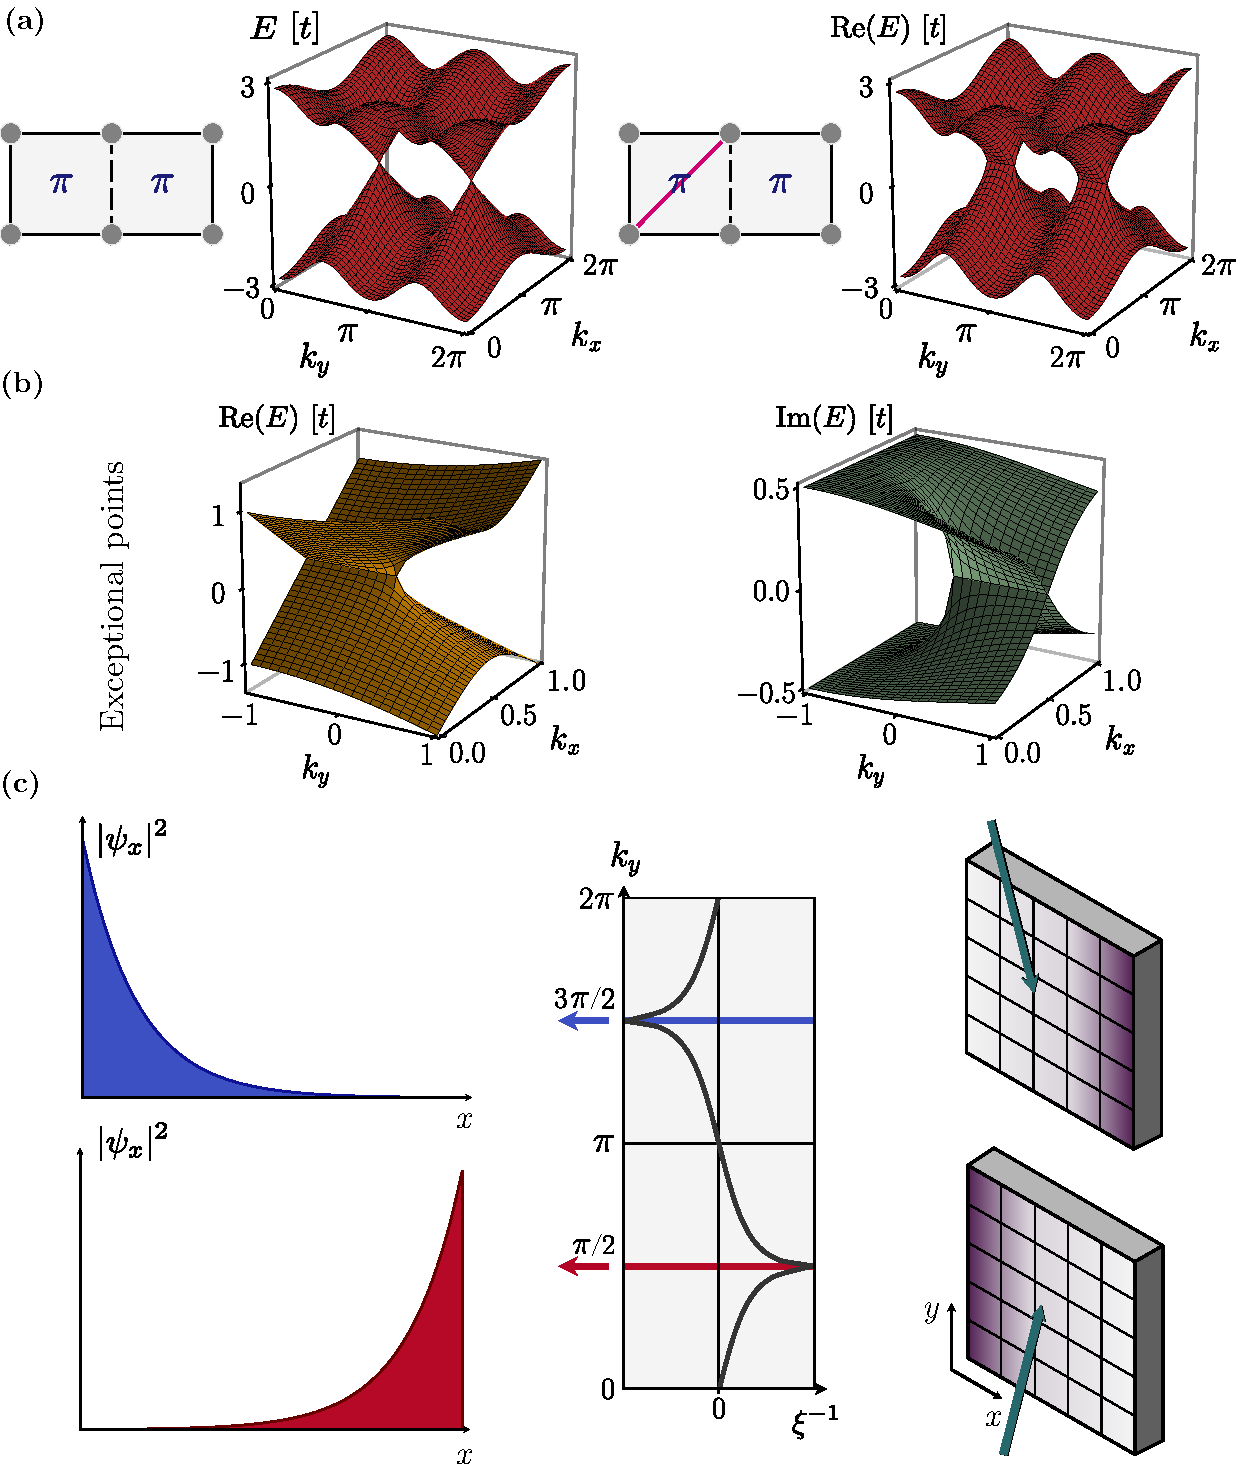
\includegraphics[width=0.95\columnwidth]{nh-theory.pdf}
\caption[Theory of the reciprocal skin effect]{\textbf{(a)} Left: unit cell and spectrum of the $\pi$-flux model defined in Eq.~\eqref{eq: pi flux} with periodic boundary conditions. Solid and dashed lines correspond to hopping amplitudes $t$ and $-t$, respectively. Bands touch in two Dirac points. Right: $\pi$-flux model with a non-Hermitian diagonal hopping (pink) included, as defined in Eq.~\eqref{eq: non-Hermitian H}. Each Dirac point splits into a pair of exceptional points. \textbf{(b)} Real and imaginary part of eigenvalues in the vicinity of an exceptional point, at which two complex eigenvalues are degenerate. \textbf{(c)} Schematic of the reciprocal skin effect for OBC in $x$ and PBC in $y$ direction: near two opposite momenta, $k_y= \pi /2$ and $k_y=3 \pi /2$, all eigenstates are exponentially localized with localization length $\xi$ to the left and right of the system, respectively. At $k_y=0, \, \pi$ the modes are completely delocalized. Right: The reciprocal skin effect could serve as a direction detector for incident electromagnetic waves: dependent on the propagation direction and polarization, a voltage will build up on the left or right edge of the system, as shown schematically.}
\label{fig: 1}
\end{figure}

\begin{figure}[H]
\centering
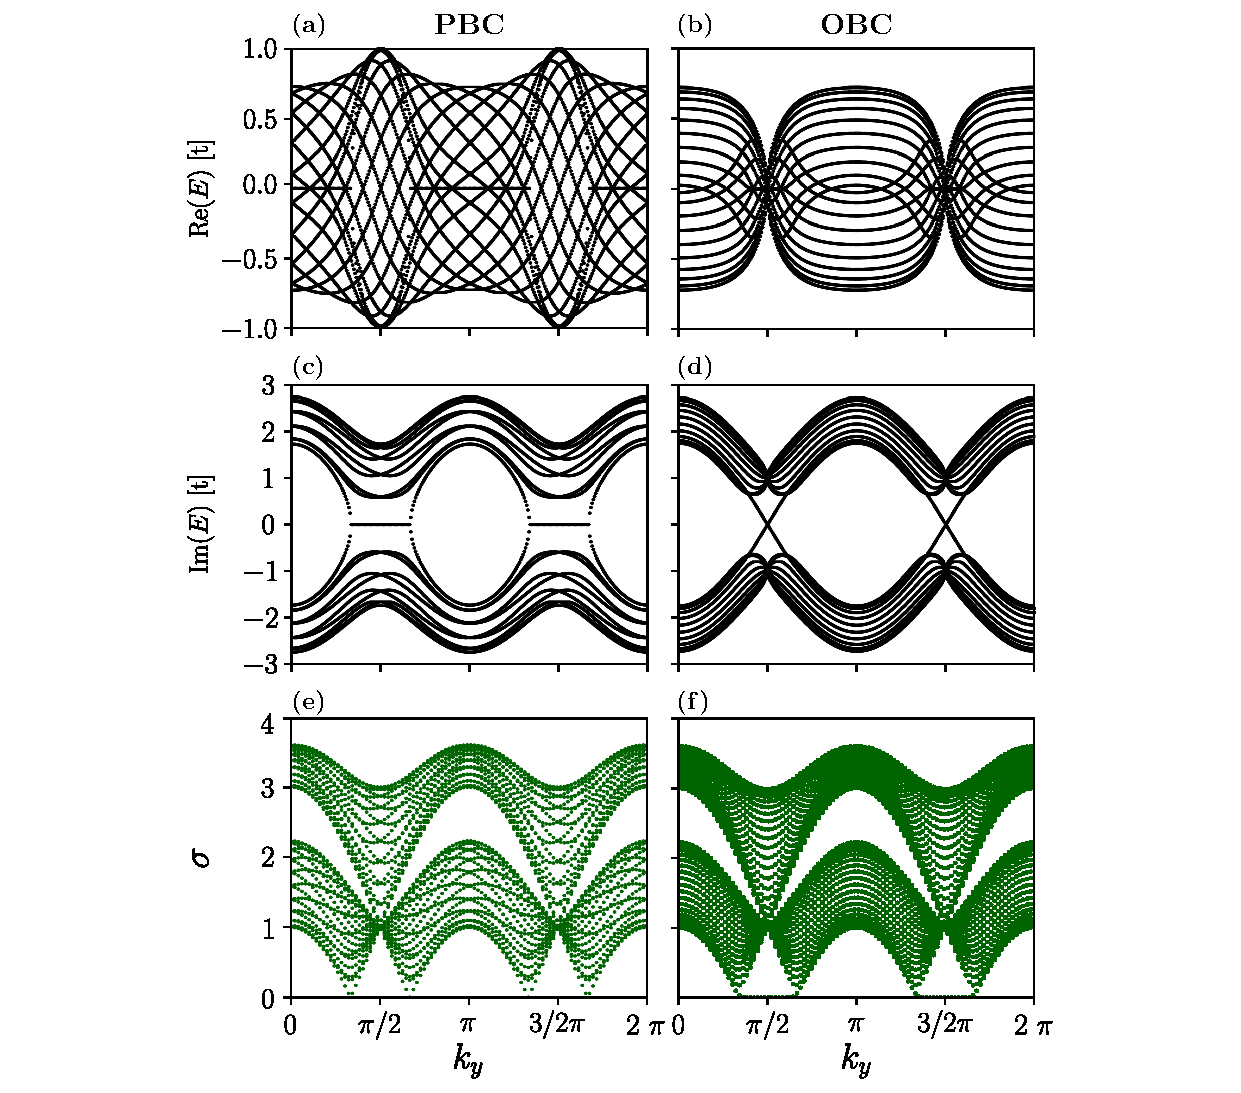
\includegraphics[width=0.95\columnwidth]{nh-piflux.pdf}
\caption[Numerical calculation of the complex eigenspectrum and singular value decomposition of the non-Hermitian $\pi$-flux model]{Numerical calculation of the complex eigenspectrum and singular value decomposition of the non-Hermitian $\pi$-flux model with $r = 1$. Real part of the \textbf{(a)} PBC and \textbf{(b)} OBC spectrum, imaginary part of the \textbf{(c)} PBC and \textbf{(d)} OBC spectrum, together with the singular values for \textbf{(e)} PBC and \textbf{(f)} OBC. Non-perturbative change in the energy spectra manifests the breakdown of bulk-boundary correspondence associated with the extensive localization of eigenmodes. However, the singular spectra closely resemble each other, with the only difference in additional zero singular values around $k_y = \pi / 2$ and  $k_y = 3 \pi / 2$ observed for OBC. This indicates a change in the band gap topology.}
\label{fig:num_spectrum}
\end{figure}

Due to the inclusion of non-Hermitian terms, topological states can emerge in the full Hamiltonian, which are not present in the initial Hermitian $\pi$-flux model. Our discussion closely follows Ref.~\cite{Shunyu2018prl}. To study the topological aspects in a system with $N$ unit cells, we perform a \textit{non-unitary} transformation $\mathcal{H}_{k_y}' = S^{-1} \mathcal{H}_{k_y}S$ with $S= \text{diag}(1, a,a,a^2,a^2, \dots,a^{N-1}, a^N)$ and $a= \sqrt{(1-i r_x -r_y)/(1-i r_x +r_y)}$, where open boundary conditions are implied. The transformed Hamiltonian under application of PBC can be rewritten as a reciprocal SSH chain with complex coefficients,
\begin{equation}
\mathcal{H}_{k_y}' =  \big[t_0+\cos(k_x) \big]\,\sigma_x + \big[\sin(k_x) \big]\,\sigma_y + m \, \sigma_z,
\end{equation}
where $t_0 = \sqrt{(1-i r_x)^2-r_y^2} \in \mathbb{C}$. We point out that the transformation has to be firstly performed on the Hamiltonian with OBC and after that the PBC are applied. This is not equivalent to the case, when the transformation is done for the already periodic system. SSH-type edge modes exist on both edges of the system, if $|t_0|<1$, which translates to a topological regime for
\begin{equation}
\cos(k_y) < \sqrt{\frac{1}{2} - \left(\frac{r}{2}\right)^2},
\end{equation}
parametrized by the momentum $k_y$. The bulk spectrum of $\mathcal{H}_{k_y}'$ is gapped, if either $t_0 \neq 1$ or $m\neq 0$. The gap closes at $r=\sqrt{2}$ for $k_y = \pi/2$, which marks the topological phase transition in $r$. If $r\geq\sqrt{2}$, there are no topological states. As the spectra of $\mathcal{H}_{k_y}'$ and $\mathcal{H}_{k_y}$ are identical, the total Hamiltonian with OBC in the $x$-direction exhibits a bulk gap for all $k_y$ in the boundary Brillouin zone for $r\neq \sqrt{2}$. The topological phase transition does in general not occur at the PBC band closings, but is instead parametrically displaced due to the non-Hermiticity. Only for the special choice of $r=1$, the two conditions coincide, resulting in topological transitions at the PBC exceptional points for $k_y = \pm \pi/3, \pm 2 \pi /3$. The topological boundary modes disperse with $\pm m = \pm 2 \, \cos(k_y)$ and assume a linear dispersion at the original location of the Dirac crossings in the non-Hermitian model at $k_y = \pi/2, 3\pi/2$ in the boundary Brillouin zone. Note that the bulk is gapped at those points, while the edge states cross at zero energy. The analysis shows that SSH-type modes can coexist with skin modes in the non-Hermitian model with open boundaries along $x$.


\subsection{Reciprocal skin effect}
We proceed to consider the Hamiltonian~\eqref{eq: non-Hermitian H} with OBC in the $x$-direction, which leaves $k_y \in [0,2\pi]$ as a well-defined momentum, and denote $\tilde{\mathcal{H}}(k_y)$ as the Hamiltonian for a ribbon geometry. While $\tilde{\mathcal{H}}^{\mathrm{T}} (k_y) = \tilde{\mathcal{H}}(-k_y)$ guarantees reciprocity of the full system, each instance of $\tilde{\mathcal{H}}(k_y)$ \textit{locally} breaks reciprocity for a fixed $k_y$ when seen as a purely one-dimensional model, except for $k_y = - k_y$. The reciprocal skin effect is characterized by a $k_y$-dependence of this localization property. The bulk modes of the Hamiltonian with OBC in the $x$ direction are localized on one boundary of the system with $\psi_x \sim e^{-x/\xi}$, where 
\begin{equation}
\xi^{-1} = \frac{1}{4} \ln\left(\frac{1+r^2+2 r \sin(k_y)}{1+r^2-2 r \sin(k_y)}\right).
\label{eq:local_leng}
\end{equation}
We illustrate the localization length $\xi$ in Fig.~\ref{fig: 1}~(c). $\xi$ is positive, if $k_y \in \, (0,\pi)$ and negative if $k_y \in \, (\pi,2\pi)$ in the boundary Brillouin zone with open boundaries along $x$. This leads to left edge localized modes, if $k_y \in \, (0,\pi)$ and to right edge localization, if $k_y \in \, (\pi,2\pi)$. The strongest localization is found at the original positions of the Dirac crossings in the boundary Brillouin zone,  $k_y = \pi/2, 3\pi/2$.  At those points, $\xi$ vanishes for $r\rightarrow 1$ leading to infinite localization, which is accompanied by exceptional points at finite energy in the OBC spectrum of the model. The localization length inherits the reciprocal symmetry from the full model as $\xi(-k_y) = -\xi(k_y)$. A state at $k_y$ has a reciprocal partner mode at $-k_y \mod 2\pi$, which possesses the same absolute localization length, but is localized on the opposite edge. Combining those partners preserves reciprocity in the full model. For $k_y = 0$ or the self-symmetric momenta, the localization length diverges. The corresponding bulk eigenstates are delocalized and bulk-boundary correspondence is restored. This can be observed in Fig.~\ref{fig:num_spectrum}, where at $k_y = 0$ and $k_y = \pi$, the PBC and OBC spectra match and they do not form any loops in the complex plane~\cite{okuma2019topological, zhang2019correspondence}. 

It is important to highlight that the reciprocal skin effect in two dimensions is fundamentally different to a doubled and reciprocity-enhanced 1D skin effect, as realized for instance by two reciprocity-reversed Hatano-Nelson chains~\cite{hatano-nelson}. To conceptualize this, consider an analogy to the 2D Chern insulator and the 3D Weyl semimetal~\cite{Shuichi_Murakami_2007}. Coupling two time-reversed copies of a Chern insulator with chiral edge states constitutes the $\mathbb{Z}_2$ topological insulator with helical edge states and restores time-reversal symmetry~\cite{PhysRevLett.95.146802}. In a similar fashion, one can create an overall reciprocal system out of two Hatano-Nelson chains, whose exponentially localized modes are not protected by symmetry. Only by the demand of additional symmetries which square to $-1$, the precise notion of a $\mathbb{Z}_2$ skin effect is defined~\cite{okuma2019topological}. In distinction to this symmetry enhancement, we consider dimensional enhancement. The Weyl semimetal in 3D can be composed of 'slices' of momentum space, which are characterized by a 2D Chern insulator. By analogy, we extend the 1D (non-reciprocal) skin effect to two dimensions, arriving at the reciprocal skin effect, with momentum space slices that host the 1D skin effect. Slices at opposite momenta are connected by the reciprocity transformation. In contrast to one-dimensional systems, hybridization of those reciprocal partners is intrinsically prevented by the translational symmetry of the two-dimensional system.

\subsubsection{Theoretical derivation of the skin effect via non-unitary transformation}
Here, we show the explicit derivation of the reciprocal skin effect. We expand the Hamiltonian in Eq.~\eqref{eq: non-Hermitian H} to linear order in the momentum deviations $\delta k_y$ around the exceptional points and in $r$ (\ie, we drop a term $\mathcal{O}(r\,\delta k_y)$). Let us denote by $H^{(\pm)}_{x\alpha,x'\alpha'}(\delta k_y)$ the matrix elements for the such expanded strip Hamiltonian,
where $x,x'=1,\cdots, L$ labels the unit cell across the strip and $\alpha,\alpha'\in\{1,2\}$ refers to the two sublattices. We show now that, under OBC (but not PBC), this non-Hermitian Hamiltonian is related to a pair of well-known Hermitian Hamiltonians by \emph{non-unitary} transformations. Our discussion closely follows Ref.~\cite{Shunyu2018prl}. The transformation (setting $t=1$)
\begin{equation}
O_{x,x'}^{(\pm)}=\delta_{x,x'}\left(\sqrt{\frac{1\mp r}{1\pm r}}\right)^x M^{(\pm)}(r),
\end{equation}
with $M^{(\pm)}(r)$ an appropriate $2 \times2 $ non-singular matrix acting on the sublattice space, maps  $\tilde{H}^{(\pm)}(\delta k_y)=\left(O^{(\pm)}\right)^{-1}H^{(\pm)}(\delta k_y)O^{(\pm)}$, with
\begin{equation}
\begin{aligned}
\tilde{H}^{(\pm)}_{x,x'}(\delta k_y)
=&\,
\delta_{x,x'}
\begin{pmatrix}
2\delta k_y&-\sqrt{1-r^2}\\
-\sqrt{1-r^2}&-2\delta k_y
\end{pmatrix}
-
\begin{pmatrix}
0&\delta_{x',x+1}\\
\delta_{x',x-1}&0
\end{pmatrix}.
\end{aligned}
\label{eq: SSH Hamiltonian}
\end{equation}

For $\delta k_y=0$, Eq.~\eqref{eq: SSH Hamiltonian} is the tight-binding Hamiltonian for a dimerized chain, known as the Su-Schrieffer-Heeger model (see Fig.~\ref{fig: nonunitarytransform}). For $-1<r<1$, $r\neq0$, the chain is bulk insulating but has one SSH-type midgap state localized at each end of the chain. Its bulk states are of delocalized Bloch character, while the end states are exponentially localized with a ratio $\tilde{\psi}_{x,\alpha}/\tilde{\psi}_{x\pm1,\alpha}=\sqrt{1-r^2}$ of wave function amplitudes on neighboring lattice sites. We denote by $\psi_{x,\alpha}(\delta k_y)$ and $\tilde{\psi}_{x,\alpha}(\delta{k_y})$ the eigenstates of $H^{(\pm)}(\delta k_y)$ and $\tilde{H}^{(\pm)}(\delta k_y)$, respectively. Finite but small $\delta k_y$ mainly has the effect of lifting the degeneracy of the SSH-type end states from eigenvalue $0$ to $\pm 2\delta k_y$. 

Being related by $O^{(\pm)}$, $\tilde{H}^{(\pm)}(\delta k_y)$ and the non-Hermitian Hamiltonian $H^{(\pm)}(\delta k_y)$ are isospectral, but their eigenstates differ in important ways. The $x$-dependent factor in $O^{(\pm)}$ turns \emph{all} the Bloch-type bulk states into exponentially localized states, with $\psi_{x,\alpha}/\psi_{x\pm1,\alpha}\approx \sqrt{2/(1\pm r)-1}$ -- which is a stronger exponential decay than that of the SSH-type end states. This implies that the two topological edge states become localized at the same end of the chain after the non-unitary transformation. Whether the localization is on the left or right edge of the system depends on the sign of $r$ and is opposite for $H^{(+)}(\delta k_y)$ and $H^{(-)}(\delta k_y)$. We conclude that on a strip geometry all eigenmodes of the model in Eq.~\eqref{eq: non-Hermitian H} are localized on one side of the sample for $k_y \sim \pi/2$ and on the opposite side for $k_y \sim 3\pi/2$. This constitutes the reciprocal skin effect, enabled by the non-Hermiticity of the Hamiltonian. 

\begin{figure}[!htbp]
\centering
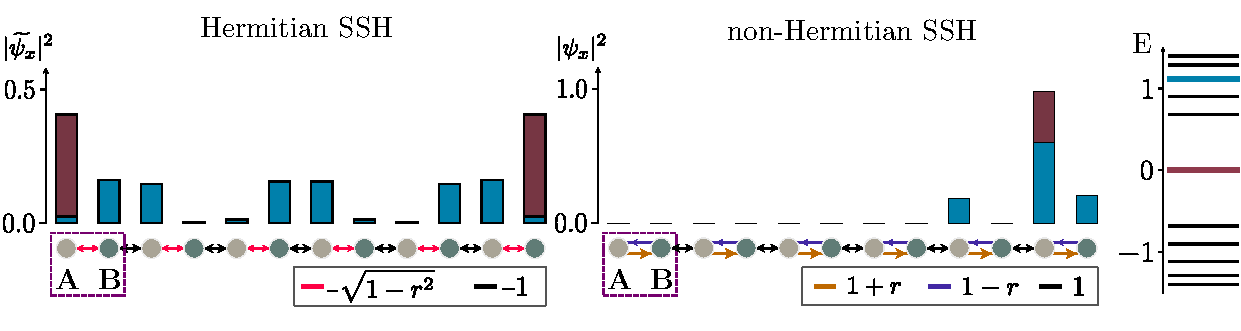
\includegraphics[width= \textwidth]{nh_ssh-chain.pdf}
\caption[Relation between the Hermitian ($r = 0$) and non-Hermitian ($r = 0.9$) dimerized chain, the SSH model.]{Relation between the Hermitian ($r = 0$) and non-Hermitian ($r = 0.9$) dimerized chain, the SSH model. The spectrum of both models is equal with open boundary conditions, including SSH-type end states. However, all states in the non-Hermitian model are localized on one side of the system. The amplitude at each lattice site for the two eigenstates marked in the spectrum on the right are plotted with the respective color.}
\label{fig: nonunitarytransform}
\end{figure}

\section{Experimental topolectrical circuit realization}
\label{sec:topocircuit}
In principle, various non-Hermitian, \ie lossy, classical systems could be deliberately tailored to study the physical effects outlined above. Topolectrical circuits in particular, however, offer an important advantage due to the only mild limitation imposed by local connectivity constraints otherwise typical to many other metamaterial settings. Most importantly, a connection between the leftmost and rightmost site of a circuit can simply be toggled on/off to change between PBC and OBC. This way, the breakdown of bulk-boundary correspondence can be studied most directly. We experimentally implemented a circuit which realizes the non-Hermitian but reciprocal model given in Eq.~\eqref{eq: non-Hermitian H} through its response function within linear circuit theory. The circuit Laplacian matrix $J (\omega)$ takes the role of the reciprocal Hamiltonian introduced above. More concretely, it connects the input currents $I_a (\omega)$ at node $a$ of the system to the voltages $V_b (\omega)$ measured at $b$ via Kirchhoff's law, represented in the frequency domain by $I_a (\omega)=J_{ab}(\omega) V_b(\omega)$.

\subsection{Laplacian formalism}
In a passive circuit network of capacitors (C), inductors (L), and resistors (R), currents and voltages are linearly related through a discretized version of the Laplacian operator as a second order spatial derivative. However, in such a circuit system, energy is not necessarily conserved as it can dissipate in an irreversible heating process occurring in resistors. In contrast to purely capacitive or inductive couplings, which oppose the \textit{change} of electric currents or voltages, a resistor opposes the \textit{flow} of an electric current and is, as such, intrinsically non-Hermitian. To be able to analyze the present circuit setup, which involves all of the passive components R, L, C, we rely on non-Hermitian linear circuit theory.

Define $V_a$ and $I_a$ to be the voltage and external input current on node $a$ of a circuit network. Using Kirchhoff's and Ohm's laws, we obtain a coupled system of differential equations for the circuit,
\begin{equation}
\dot{I}_a=\Gamma_{ab} \, \ddot{V}_b+\Sigma_{ab} \, \dot{V}_b+\Lambda_{ab} \, V_b,
\label{dotI}
\end{equation}
where $\Gamma_{ab},\Sigma_{ab}$ and $\Lambda_{ab}$ are the reduced Laplacian matrices of capacitances, conductances and inverse inductances, and the summation over repeated indices is implied. The diagonal components $a=b$ of the Laplacians are defined by 
\begin{equation}
X_{aa}=-X_{a0}-\sum_{b=1,2,\cdots}X_{ab},\qquad X\in\{\Gamma,\Sigma,\Lambda\},
\end{equation}
including the circuit elements $X_{a0}$ between node $a$ and the ground. 

A Fourier transformation of Eq.~\eqref{dotI} from the time to frequency domain results in
\begin{equation}
I_a=\left(\mathrm{i}\omega \, \Gamma_{ab}+\Sigma_{ab}-\frac{\mathrm{i}}{\omega} \, \Lambda_{ab}\right)V_b =J_{ab}(\omega) \, V_b ,
\label{I2}
\end{equation}
where we defined $J_{ab}(\omega)$ as the (grounded) circuit Laplacian~\cite{LeeTopolectrical18}. Note that $\omega$ is treated as a parameter of the system which is fixed by the external AC driving frequency. 

A natural observable in a circuit is the impedance response $Z_{a 0}$, which is the ratio of the voltage at node $a$ measured with respect to ground due to an input current $I_{j}=I_0\,\delta_{j,a}$ that enters through $a$ and exits through ground. Mathematically, $Z_{a0}$ involves the inversion of Eq.~\eqref{I2}
\begin{equation}
Z_{a0}(\omega)&= \frac{V_a}{I_0} 
= \sum_j\frac{G_{aj} \, I_i}{I_0}
= G_{aa} = \sum_n\frac{\psi_{n,a} \, \phi_{n,a}^{*}}{j_n},
\label{impedance1}
\end{equation}
where $J_{ab}(\omega)=\sum_n j_n(\omega) \psi_{n,a} \phi^*_{n,b}$ defines the spectral representation of the Laplacian with its right and left eigenvectors, $\psi_n$ and $\phi_n$. The frequency dependence of the Laplacian eigenvectors remains implicit. As the inverse of the Laplacian, the Green's function $G_{ab}(\omega)=\sum_n j^{-1}_n(\omega) \psi_{n,a} \, \phi_{n,b}^{*}$ contains the voltage response to an external current excitation and fundamentally determines both the excitation pattern of individual eigenmodes and the circuit's impedance profile with frequency. The grounding impedances are given by the diagonal elements of $G$.

The off-diagonal components of the Green's function are accessible using an arrangement of measurements similar to that of the impedance response $Z_{a 0}(\omega)$. We feed a current $I_a$ at node $a$ and measure the voltage response $V_b^{(a)}$ at all the other nodes. By repeating this for all input nodes, the Green's function can be reconstructed as
\begin{equation}
G_{a b} = \frac{V_b^{(a)}}{I_a} .
\label{eq:Greens Function Measurement}
\end{equation}
In the circuit formalism, the Green's function as a direct observable contains full information on admittance eigenvalues and eigenmodes of the Laplacian, which can be extracted through numerical diagonalization. The procedure to measure the Green's function can be simplified in periodic models using spatial Fourier transform~\cite{PhysRevB.99.161114}.

\subsubsection{Derivation of the circuit Laplacian}
\label{sec:circ-laplacian}
We realize the reciprocal skin effect in an electrical circuit whose unit cell is shown in Fig.~\ref{fig: 2}~(a), with the conceptually important elements of each plaquette shown in Fig.~\ref{fig: 2}~(b). The two-point Laplacian of a capacitor is given by
\begin{equation}
\begin{pmatrix}
I_{\text{in},1}\\I_{\text{in},2} 
\end{pmatrix}
=\mathrm{ i} \omega \left[ C 
\begin{pmatrix}
1 & -1 \\ -1 & 1
\end{pmatrix}
\right]
\begin{pmatrix}
V_1 \\ V_2
\end{pmatrix} .
\end{equation}
Omitting the prefactor $\mathrm{i} \omega$ results in the symmetric and Hermitian Laplacian matrix. The Laplacian for an inductor takes a similar form
\begin{equation}
\begin{pmatrix}
I_{\text{in},1}\\I_{\text{in},2} 
\end{pmatrix}
= \mathrm{i} \omega \left[ - \frac{1}{\omega^2 L}
\begin{pmatrix}
1 & -1 \\ -1 & 1
\end{pmatrix}
\right]
\begin{pmatrix}
V_1 \\ V_2
\end{pmatrix} ,
\end{equation}
that differs in the frequency-dependent admittance prefactor and, importantly, in the overall sign. At the resonance frequency $\omega_0 = 1/\sqrt{L C}$ of an $LC$ resonator, the inductor effectively acts a negative capacitor, where $-1/(\omega_0^2 L) = -C$ in front of the Laplacian matrix. Therefore, one circuit plaquette of the $\pi$-flux model consists of three capacitors (representing $t$) and an inductor (representing $-t$ at resonance), all of which are Hermitian and reciprocal. At nodes of sublattice $A$, the diagonal contributions in the Laplacian add to $4 C$, whereas for $\omega = \omega_0$ the capacitive and inductive contributions cancel each other in the diagonal term at sublattice $B$. To avoid the sublattice asymmetry contributing to a $\sigma_z$ term, we ground nodes of type $A$ with an inductor $L_g \approx L/4$ such that the diagonal contribution to the Laplacian vanishes for both sublattices at resonance frequency.
In total, the circuit Laplacian in momentum space is given by
\begin{equation}
\begin{aligned}
J_\pi(k_x,k_y&) = \mathrm{i} \omega \bigg[
	-\begin{pmatrix}
	2 C \cos(k_y)  & C(1 + e^{-\mathrm{i} k_x}) \\
	C(1+e^{\mathrm{i} k_x}) & 2/(\omega^2 L) \cos(k_y) 
	\end{pmatrix}  \\
	&+
	\begin{pmatrix}	
	4 C - 1/(\omega^2 L_g) & 0 \\
	0 & 2 C - 2/(\omega^2 L)
	\end{pmatrix}
\bigg]
\end{aligned}
\end{equation}
resembling the $\pi$-flux tight-binding model for $\omega \rightarrow \omega_0$, where the second term vanishes. Additional to $J_\pi(k_x,k_y)$, we introduce a resistor connecting nodes $A$ and $B$ of adjacent unit cells in the $y$-direction (see Figs.~\ref{fig: 2}~(a) and (b)). Its admittance representation reads
\begin{equation}
\begin{pmatrix}
I_{\text{in},1}\\I_{\text{in},2} 
\end{pmatrix}
= \mathrm{i}\omega \left[ - \frac{i}{\omega R}
\begin{pmatrix}
1 & -e^{\mathrm{i} k_y} \\ -e^{-\mathrm{i} k_y} & 1
\end{pmatrix}
\right]
\begin{pmatrix}
V_1 \\ V_2
\end{pmatrix}  \equiv J_{r} \begin{pmatrix}
V_1 \\ V_2
\end{pmatrix}.
\end{equation}
The total Laplacian is given by $J = J_{\pi} +J_r$. With $\mathrm{i} \omega$ factored out, the added Laplacian $J_r$ is non-Hermitian and breaks time-reversal symmetry. For an arbitrary circuit network described by $J(k_y,k_y)$, reciprocity is defined as $J^{\mathrm{T}} (k_x, k_y) = J(-k_x, -k_y)$. Thus, a resistor is a reciprocal circuit element. However, if one considers a fixed $k_y$ slice of the model, reciprocity is broken as $e^{\mathrm{i} k_y} \neq e^{-\mathrm{i} k_y}$ for arbitrary $k_y\neq 0,\pi$. 

\begin{figure}[H]
\centering
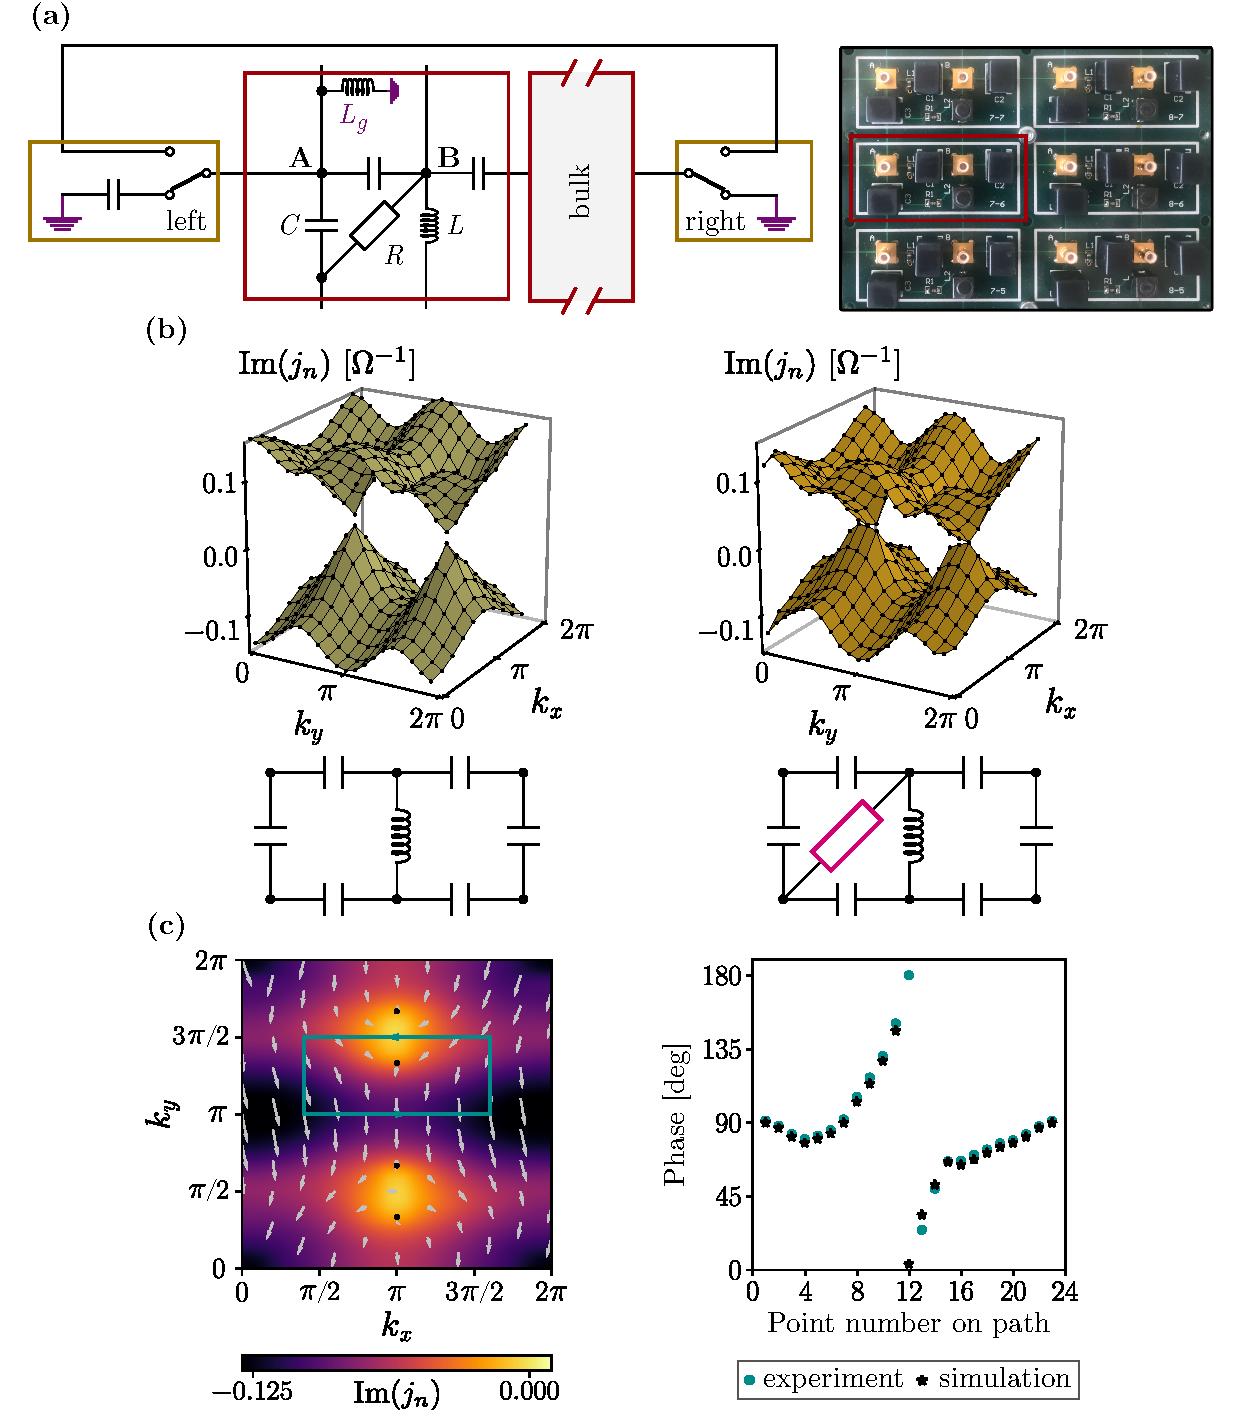
\includegraphics[width=\columnwidth]{nh-experiment.pdf}
\caption[Experimental topolectrical circuit realization of the reciprocal skin effect and exceptional points]{Experimental topolectrical circuit realization of the reciprocal skin effect and exceptional points. \textbf{(a)} Bulk unit cell and boundary terminations of the circuit, together with a photography of six unit cells of the assembled circuit board. Section~\ref{sec:circ-laplacian} details the connection of this circuit cell to the lattice model in Eq.~\eqref{eq: non-Hermitian H} using the Laplacian formalism. \textbf{(b)} Measured spectra with PBC of the circuit Laplacian and schematic unit cell of the circuit that corresponds to the $\pi$-flux model (left) and the non-Hermitian model (right) from Eq.~\eqref{eq: non-Hermitian H} (cf. Fig.~\ref{fig: 1}~(a)). Only the imaginary part of the eigenvalues is plotted. The formation of a branch cut from the Dirac point is visible, the ends of which are host to exceptional points. \textbf{(c)} Left: Imaginary part and phase of the band with smaller imaginary part. The phase of the eigenvalue along the path indicated is plotted in the right panel. It shows a clear jump by $\pi$, indicative of an enclosed exceptional point. Stars denote a \textsc{LTspice} simulation of the circuit, while dots correspond to the measured spectrum.}
\label{fig: 2}
\end{figure}

\subsection{Non-Hermitian topolectric circuit}
In a Hermitian circuit, all eigenvalues of $J(\omega)$ are purely imaginary ($\mathrm{i}J(\omega)$ is a Hermitian matrix), while the inclusion of resistors generates complex eigenvalues. Interpreting $J (\omega)$ at a fixed frequency $\omega_0$ as a hopping matrix, one observes that the sign change of $t$ necessary to implement the $\pi$-flux model is achieved by connecting one of the three bonds surrounding a plaquette in a square lattice with an inductor and three with a capacitor (consult Fig.~\ref{fig: 2}~(a) and~(b)). We fabricated a circuit with $10 \times 20$ unit cells using this model.

Assuming translation invariance (realized to the accuracy of the circuit element specifications), we can represent the voltages and input currents in terms of Fourier modes in reciprocal space. This leads to the $k$-space representation of the Laplacian as well as its voltage eigenmodes and allows for the definition of a complex-valued admittance band structure. The latter can be understood as a complex mapping from wave vector $k$ to admittance eigenvalues of the Laplacian. In a measurement, we can decompose the voltage response to an external current excitation and find the eigensystem of the Laplacian for both periodic and open boundary conditions. Fig.~\ref{fig: 2}~(b, left) shows the measured bands including the two Dirac-cone band touchings expected for the $\pi$-flux model. The Dirac points are broadened into branch cuts, each of which spans between a pair of exceptional points. To demonstrate this, we plot the phase of the eigenvalue for the band $j_n(\omega_0,k_x,k_y)$ with smaller imaginary part along a closed path in Fig.~\ref{fig: 2}~(c). The observed winding and phase jump by $\pi$ is direct evidence that the path encircles an exceptional point in momentum space, which is topologically stable exactly through this half-integer winding number of the band eigenvalue around it.

Having confirmed that the circuit realizes the desired physics of an exceptional point band structure with PBC, we now present measurements with OBC in $x$-direction to demonstrate the reciprocal skin effect. Edge terminations are chosen such that the circuit grounding does not introduce undesired off-sets due to a change in the total node conductance at the edge sites, see Fig.~\ref{fig: 2}~(a). The measured $k_y$-resolved spectra are shown in Fig.~\ref{fig: 2a}, in comparison to an equivalent representation of the data for PBC. The eigenvalues with small imaginary part around $k_y\sim \pi/2, 3\pi/2$ indeed show the expected reorganization from a spectrum with two exceptional points in the bulk towards much fewer states with OBC -- a breakdown of the Hermitian bulk-boundary correspondence. The reciprocal skin effect is encoded in the coloring of the data points: red and blue dots correspond to right and left localized eigenstates. (Note that through the measurement of the full matrix $J(\omega_0)$ not only do we have access to its spectrum, but also to all of its eigenstates.). The degree of localization of eigenstates is quantified by the inverse participation ratio (IPR)~\cite{ipr}. Remarkably, \emph{all} states near $k_y\sim \pi/2$ are right-localized, while \emph{all} states near $k_y\sim 3\pi/2$ are left-localized.

\begin{figure}[!htbp]
\centering
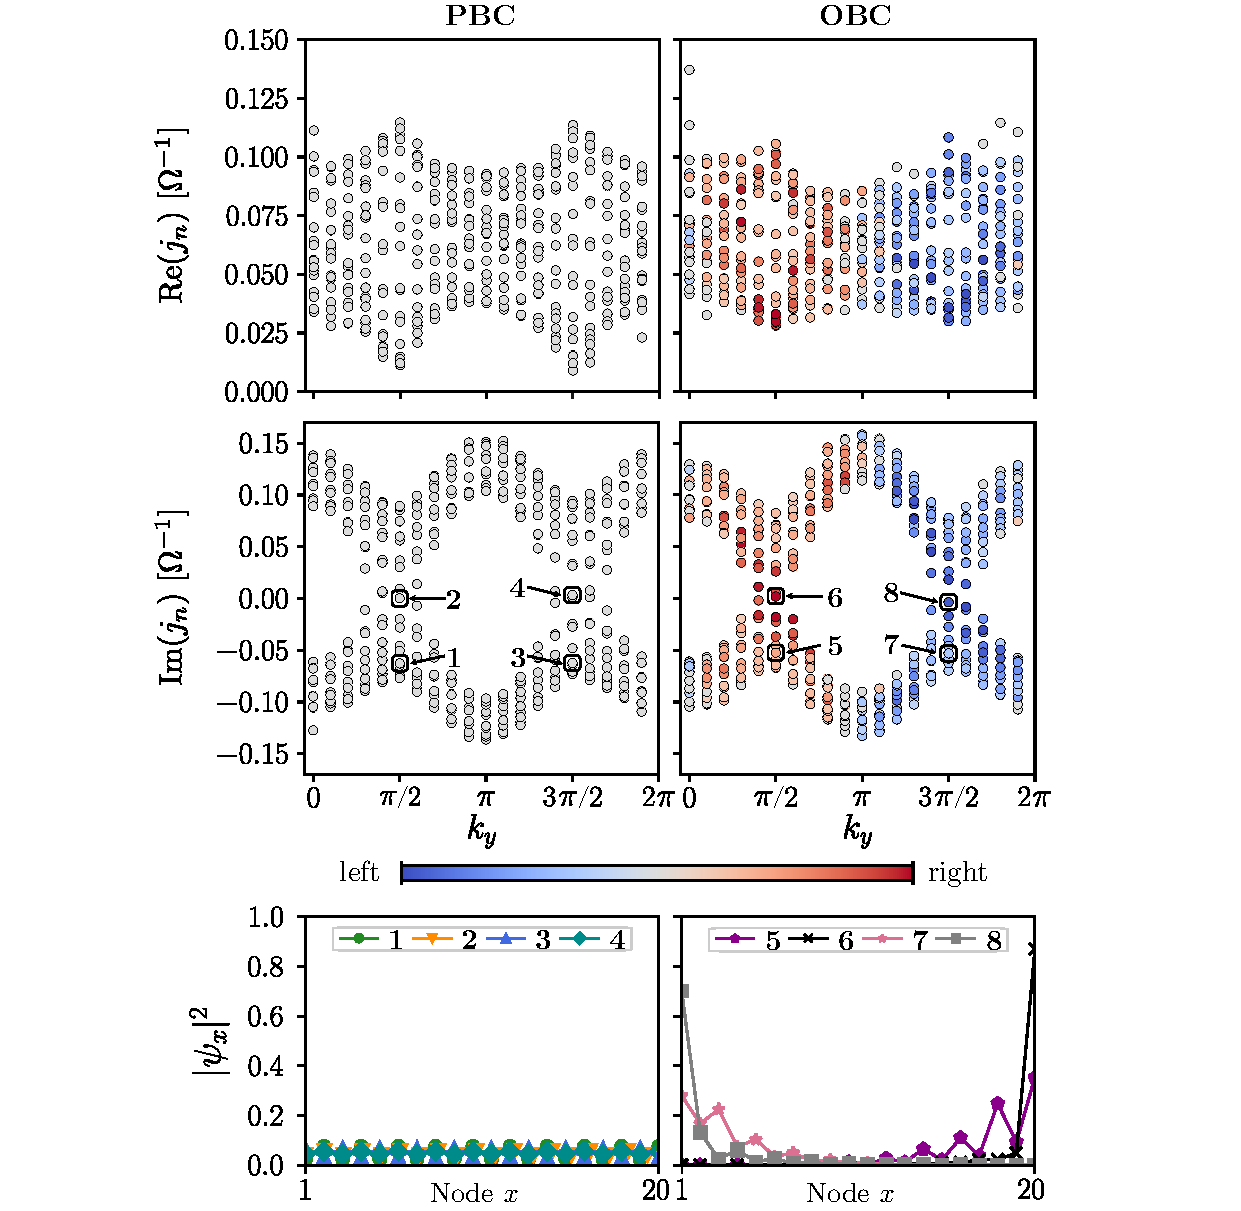
\includegraphics[width=\columnwidth]{nh-experiment-2.pdf}
\caption[Measured spectra of the circuit Laplacian as a function of $k_y$ for OBC and PBC along the $x$ direction]{Measured spectra of the circuit Laplacian as a function of $k_y$ for OBC and PBC along the $x$ direction. Localization properties of each eigenstate are indicated by color and determined from the inverse participation ratio. The bottom panel shows the localization properties of representative individual eigenstates at $k_y = \pi /2$ and $k_y = 3 \pi /2$, both for PBC and OBC. The fact that \emph{all} OBC and PBC eigenstates differ non-perturbatively constitutes the reciprocal skin effect, with those around $k_y \sim \pi / 2$ right-localized and those around $k_y \sim 3 \pi /2$ left-localized.}
\label{fig: 2a}
\end{figure}

\subsection{Representation of the Laplacian spectra in the complex plane}
In addition, we present an alternative representation of the complex spectra of the circuit Laplacian, both theoretical and experimental. For this, we consider $k_y$ as a parameter and plot for each fixed $k_y$ the set of eigenvalues in the complex plane $\mathrm{Re}(j_n)$-$\mathrm{Im}(j_n)$. This generates a two-dimensional closed surface, as shown in Fig.~\ref{fig: S2}~(a) for PBC. As a function of $k_y$, the eigenvalues trace out either a single circle or two circles in the $\mathrm{Re}(j_n)$-$\mathrm{Im}(j_n)$ plane. The transitions between these two topologically distinct situations are exceptional points. The planes $k_y=0$ and $k_y=\pi$ are special, because the path traced out in the complex plane as a function of $k_x$ is reciprocal on them. Therefore, it collapses into lines on which each non-end point is visited two times as $k_x$ is varied~\cite{PhysRevB.99.201103}.

Since we have two pairs of exceptional points, the two-dimensional eigenvalue surface in $k_y$-$\mathrm{Re}(j_n)$-$\mathrm{Im}(j_n)$ space has genus three\cite{lee2018tidal}. We can plot the experimental spectra of $J(\omega_0)$ in a similar fashion, shown in Fig.~\ref{fig: S2}~(c). We observe, for PBC, a clear change between slices at constant $k_y$ with a single circle and two circles in the complex plane of eigenvalues. This strongly indicates the presence of exceptional points between these two slices. Moreover, we note that the two cases -- at $k_y = \pi /2$ and $k_y = 3 \pi /4$ -- presented in Fig.~\ref{fig: S2}~(b) exhibit the skin effect as there exist base energies such that the complex eigenspectrum has a non-trivial winding number~\cite{okuma2019topological, zhang2019correspondence}.

\begin{figure}[!htbp]
\centering
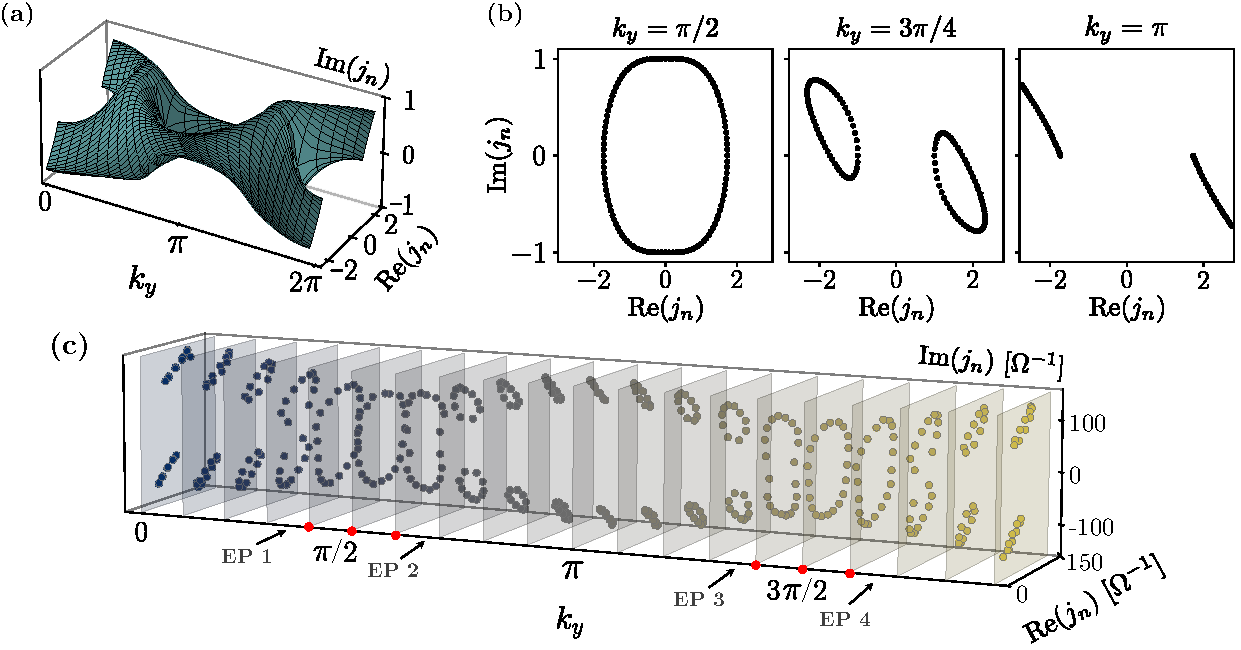
\includegraphics[width=\textwidth]{nh_circuit_pbc.pdf}
\caption[Representation of the circuit Laplacian spectra for periodic boundary conditions in the complex plane as a function of $k_y$]{Representation of the circuit Laplacian spectra for PBC in the complex plane as a function of $k_y$. \textbf{(a)} Theoretically computed spectrum showing a genus three surface with four exceptional points. \textbf{(b)} Slice plots obtained from \textbf{(a)} for three different $k_y$. \textbf{(c)} Measured spectra, where each of the four transitions from a single circle in the complex plane to two circles marks an exceptional point (EP1--EP4) as a function of $k_y$. }
\label{fig: S2}
\end{figure}

\subsection{Response of the reciprocal skin-effect circuit to bulk perturbations}
\label{sec: response}
A distinct feature of the reciprocal skin effect, which may lead to applications for polarization detection of electromagnetic waves, is the response to the circuit to perturbations in the bulk. From Eq.~\eqref{I2} we deduce that the voltage response at site $a$ to a driving current at frequency $\omega$ is given by
\begin{equation}
V_a=G_{ab}(\omega)I_b.
\end{equation}
Since our circuit has finite resistivity, $J_{ab}(\omega)$ has no zero eigenvalues at real frequencies, and can therefore be readily inverted. To model the experimental situation, we consider PBC in $y$-direction and OBC in $x$-direction. We then apply a minimal driving current to two bulk sites aligned along the $y$-direction, where we assign the current at one site a $+\pi/2$ ($-\pi/2$) phase shift with respect to the current at the other site. We therefore expect the current to excite the circuit Laplacian eigenstates at $k_y = \pi/2$ ($k_y = 3\pi/2$), which are right (left) localized in $x$-direction due to the reciprocal skin effect. Fig.~\ref{fig: S3} shows the theoretically calculated response of the circuit that is obtained by inverting the real-space version of the Hamiltonian given by Eq.~\eqref{eq: non-Hermitian H}. We find that the two driving current patterns indeed lead to non-local voltage responses at the far right (left) of the circuit. The reciprocal skin effect could therefore be the basis of a polarization detection device for electromagnetic radiation.

\begin{figure}[!htbp]
\centering
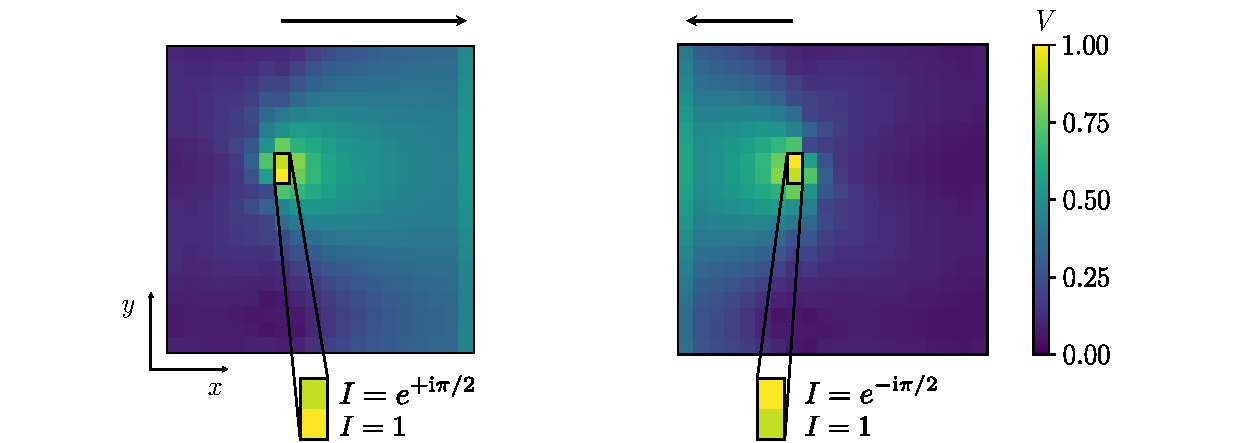
\includegraphics[width=\textwidth]{nh_time-evol.pdf}
\caption[Reciprocal skin effect voltage response due to a localized bulk driving current with phase shift]{Reciprocal skin effect voltage response due to a localized bulk driving current with phase shift. The sites where the current is applied are framed in black, the zoom-ins show how the relative phase is implemented. Importantly, for a phase shift of $+\pi/2$ ($-\pi/2$) we find a non-local voltage response at the far right (left) side of the circuit with OBC, which is absent for phase shifts $0$ and $\pi$. The arrows show the direction of voltage accumulation.}
\label{fig: S3}
\end{figure}